\documentclass[11pt,oneside]{fithesis2}
\usepackage[english]{babel} % package for multilingual support
\usepackage[utf8]{inputenc} % Windows OS encoding
\usepackage[T1]{fontenc}
\usepackage[resetfonts]{cmap}
\usepackage{lmodern}
\usepackage{graphicx}

\usepackage{listings}
\usepackage{xcolor}

\definecolor{mygray}{rgb}{0.5,0.5,0.5}

\definecolor{listingbg}{RGB}{245,245,245}
\lstset{
	basicstyle=\footnotesize\ttfamily,
	captionpos=b,
	backgroundcolor=\color{listingbg},
	framesep=4pt,
	frame=single,
	breaklines=true,
	rulecolor=\color{listingbg},
	aboveskip=10pt
}

\renewcommand\lstlistingname{Code snippet}
\renewcommand\figurename{Figure}

\usepackage[unicode=true,      
            plainpages=false,
            pdfpagelabels,
	 pdftitle={Security analysis of document protections},
            pdfauthor={Martin Bajanik},
            colorlinks=true,
            linkcolor=black, 
            citecolor=black,
            ]{hyperref}

\thesistitle{Security analysis of document protections} % enter thesis title
\thesissubtitle{Master's thesis}
\thesisstudent{Martin Bajaník} % name of the author
\thesiswoman{false} % defines author’s gender
\thesisfaculty{fi}
\thesisyear{autumn 2014}
\thesisadvisor{RNDr. Jiří Kůr, Ph.D.} % fill in advisor’s name
\thesislang{en}

\begin{document}
\FrontMatter
\ThesisTitlePage

\begin{ThesisDeclaration}
\DeclarationText
\AdvisorName
\end{ThesisDeclaration}

\begin{ThesisThanks}
Thanks ...
\end{ThesisThanks}

\begin{ThesisAbstract}
This thesis ...  
\end{ThesisAbstract}

\begin{ThesisKeyWords}
keyword1, keyword2, ...
\end{ThesisKeyWords}

\MainMatter

\tableofcontents 
\chapter{Introduction}

\chapter{Document Protections}

\section{Confidentiality}

\section{Integrity}

\section{Authenticity}

\chapter{Proprietary vs. Open Standards}

\chapter{Office Document Cryptography Structure}

\section{Encryption} 

The structure of encrypted document files is described in detail in the \textit{Office Document Cryptography Structure specification} \cite{msoffcrypto}.

This chapter aims to provide insight into the structure with respect to the discussed topics, highlight differences between various Office versions, and discuss the security implications that result from the specified protection measures.
To provide confidentiality, Office documents can be protected by a user-specified password using the following four methods:
\begin{itemize}
\setlength\itemsep{0.1em}
\item{XOR obfuscation,}
\item{40-bit RC4 encryption,}
\item{Cryptographic Application Programming Interface (CAPI) or CryptoAPI,}
\item{ECMA-376 document encryption, which can include one of the following approaches: }
	\begin{itemize}
	\setlength\itemsep{0.1em}
	\item{standard encryption,}
	\item{agile encryption and}
	\item{extensible encryption.}
	\end{itemize}
\end{itemize}

Only the last mentioned method will be further discussed as the others are not used by any modern Office versions (2007 and above) nor considered secure with the computing power currently available. The reason why they are included in all Office versions is backward compatibility with older formats \cite{msoffcrypto}.

If standard encryption or agile encryption is used, the relevant information about cryptography used to encrypt the document is contained within a structure named \textit{EncryptionInfo}.

\subsection{Standard Encryption}

Figure \ref{keys_length} shows the structure of an ECMA-376 encrypted document highlighting the \textit{EncryptionInfo} stream and elements important for the algorithms described further. The structure is represented as a binary stream (see Appendix \ref{ei_standardstream} for a detailed description).

\begin{figure}[ht]
	\centering
	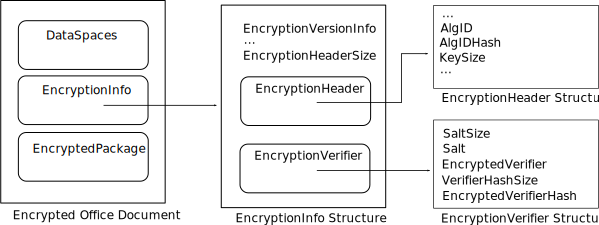
\includegraphics[width=1\textwidth]{figures/ei_struct.pdf}
	\caption{EncryptionInfo structure}
	\label{keys_length}
\end{figure}

Standard encryption describes three algorithms:
\begin{itemize}
	\setlength\itemsep{0.1em}
	\item{key derivation process,}
	\item{verifier generation process and}
	\item{password verification process.}
\end{itemize}

The key derivation process is derived from PKCS \#5: Password-Based Cryptography Version 2.0 as specified in RFC 2898 \cite{rfc2898} and the hashing algorithm used, specified in the \textit{EncryptionHeader.AlgIDHash} field, must be SHA-1. The exact steps to derive the encryption key are as follows:

\begin{enumerate}
\item{Calculate an initial password hash:}
	\begin{itemize}
		\item{$H_0 =\textit{SHA-1(salt + password)}$}
	\end{itemize}
\item{Iterate the hashing using the following approach: 
	\begin{itemize}
		\item{$H_n = \textit{SHA-1(iterator} + H_{n-1})$}
	\end{itemize}
	Variable \textit{iterator} is intially set to 0 and then incremented monotonically until 50,000 iterations have been performed.}
\item{Calculate a final hash:
	\begin{itemize}
		\item{$H_{final} = \textit{SHA-1}(H_n + block)$}
	\end{itemize}
	Variable $block$ is always $0x0000000$.}
\item{The final hash is XORed separately into the first 20-bytes of two buffers containing the bytes $0x36$ and $0x5C$ respectively. The two results of these operations are concatenated and the first $x$ bytes are considered to be the derived key, where $x$ is the key length required by the specified encryption algorithm.}
\end{enumerate}

The key is eventually used to encrypt the given document using AES in ECB mode. When attempting to decrypt the document in order to verify the correctness of a password entered, a password verifier is generated and stored within the \textit{EncryptionInfo} stream. The verifier is 16 bytes long and stored encrypted using AES in ECB mode and a key derived by the aforementioned method. In addition, an encrypted SHA-1 hash of the verifier is also stored. This information is used in the verification process as follows:

\begin{enumerate}
\setlength\itemsep{0.1em}
\item{Derive a key using the aforementioned method from the given user-password.}
\item{Decrypt the value stored in the \textit{EncryptedVerifier} field.}
\item{Decrypt the value stored in the\textit{EncryptedVerifierHash} field.}
\item{Calculate the SHA-1 hash value of the decrypted value calculated in step 2.}
\item{Compare the results of step 3 and step 4. 
	\begin{itemize}
		\item{In case the two values match the password is correct.}
	\end{itemize}}
\end{enumerate}

\begin{figure}[ht]
	\centering
	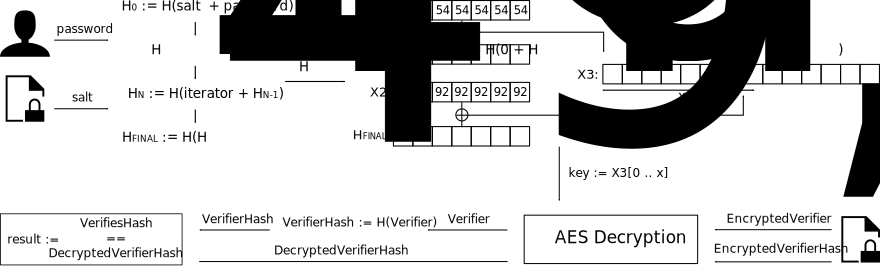
\includegraphics[width=1\textwidth]{figures/standard_encryption_scheme.pdf}
	\caption{Verification process as defined by ECMA-376 standard encryption}
	\label{standard_encryption_scheme}
\end{figure}

\subsection{Agile Encryption}

When agile encryption is used, all information about the cryptography used to encrypt the document is stored in an XML element in the \textit{XmlEncryptionDescriptor} field of the \textit{EncryptionInfo} stream. This element must conform to the XML schema namespace shown in \ref{ei_agilestream}. Agile encryption allows a wide range of possible configurations and is therefore much more complex than standard encryption discussed in the previous section. The available algorithms depend on the algorithms that can be accessed through the APIs in the Windows operating system. Microsoft Office 2007 with Service Pack 2 and above support CNG (CryptoAPI: Next Generation). The following listing shows the settings and their default values, which are configurable and change the way files are being encrypted:

\begin{itemize}
\setlength\itemsep{0.1em}
	\item{Set CNG cipher algorithm (default: AES).}
	\item{Configure CNG cipher chaining mode (default: CBC).}
	\item{Set CNG cipher key length (default: 128 bits).}
	\item{Specify encryption compatibility (default: Use next generation format).}
	\item{Set parameters for CNG context (see MSDN \cite{cng_functions}).}	
	\item{Specify CNG hash algorithm (default: SHA1).}
	\item{Set CNG password spin count (default: 100,000).}
	\item{Specify CNG random number generator algorithm (default: RNG).}
	\item{Specify CNG salt length (default: 16 bytes).}
\end{itemize}

A more detailed description of these settings can be found on the Microsoft Developer Network website\footnote{The settings and default values apply to Microsoft Office 2010 and 2013 and are identical.} \cite{plan_office_crypto}. 

Further specified are the steps necessary for deriving keys, generating initialization vectors, and generating a password key encryption structure. This structure is used to verify the correctness of the entered password when trying to open a file and it holds, encrypted, the key used to encrypt the plain-text document. Later in this chapter, this key is referred to as the intermediate key. Appendix \ref{ei_agilestream} shows the schema specifying its structure.

For the sake of completeness, it is important to mention that this structure can be represented as a \textit{CertificateKeyEncryptor} structure. The notable difference is that the intermediate key is encrypted using the public part of an X509 certificate instead of a user-supplied password. However, during the research no encrypted document was using this type of key encryptor structure nor was any information found about how to create a document using this type of protection. As a result this approach is not taken into account. 

The key derivation process is similar to the method used in standard encryption and also derived from PKCS \#5 \cite{rfc2898}:

\begin{enumerate}
\item{Calculate an initial password hash:}
	\begin{itemize}
		\item{$H_0 =\textit{H(salt + password)}$}
	\end{itemize}
\item{Iterate the hashing using the following approach:}
	\begin{itemize}
		\item{$H_n = \textit{H(iterator} + H_{n-1})$}
	\end{itemize}
\item{Calculate a final hash:}
	\begin{itemize}
		\item{$H_{final} = \textit{H}(H_n + blockKey)$}
	\end{itemize}
\item{If the length of $H_{final}$ is smaller than the key length specified in the \textit{EncryptionInfo}, then the key must be padded by appending bytes with a value of $0x36$. If it is longer, it is truncated to the correct length.}
\end{enumerate}

Note that, unlike in standard encryption, $H()$ is not a fixed hashing algorithm and the $block$ variable depends on the purpose of the key that is being derived. Another difference is that $H_{final}$ is the final key.

Initialization vectors are generated as shown in the following steps:
\begin{enumerate}
	\item{If a \textit{blockKey} is provided the IV is:}
	\begin{itemize}
		\item{$H(KeySalt + blockKey)$}
	\end{itemize}
	\item{If a \textit{blockKey} is not provided, then the IV is the \textit{KeySalt}.}
	\item{Depending on the length, the IV is either padded by appending bytes with the value of $0x36$ or truncated to \textit{blockSize} (corresponding to the encryption algorithm specified) bytes.}
\end{enumerate}

\textit{KeySalt} is specified in the document's \textit{EncryptionInfo} and again, the \textit{blockKey} is determined by the IV's purpose.

To understand how the password key encryptor is generated, it is necessary to describe the meaning of some of its elements:

\begin{itemize}
\setlength\itemsep{0.1em}
	\item{\textbf{encryptedVerifierHashInput} -- a random array of bytes encrypted using a key derived using the user-supplied password and a fixed \textit{blockKey}: $0xfe, 0xa7, 0xd2, 0x76, 0x3b, 0x4b, 0x9e, 0x79$.} 
	\item{\textbf{encryptedVerifierHashValue} -- a hash of the plain-bytes of \textit{encryptedVerifierHashInput} encrypted using a key derived using the user-supplied password and a fixed \textit{blockKey}: $0xd7, 0xaa, 0x0f, 0x6d,$ $0x30, 0x61, 0x34, 0x4e$.}
	\item{\textbf{encryptedKeyValue} -- a random array of bytes encrypted using a key derived using the user-supplied password and a fixed \textit{blockKey}: $0x14, 0x6e, 0x0b, 0xe7, 0xab, 0xac, 0xd0, 0xd6$. This element represents the intermediate key.}
\end{itemize}

In addition to confidentiality, agile encryption also provides structures that are used to verify the integrity of encrypted files. These structures are stored in the \textit{EncryptionInfo's DataIntegrity} element. The process of generating this element is further described in \ref{data_integrity}. 

As a deduction from the aforementioned steps a randomly generated key is used to encrypt the plain-text content of the documents. Unlike in standard encryption where the final encryption key was directly derived from the user-supplied password. The specification does not mention anything about how this intermediate key should be generated. In case the key is not generated using a CSPRNG (cryptographically secure pseudorandom number generator), then an implementation specific weakness is introduced and presents a serious flaw in the encryption process. 

\subsection{Extensible Encryption} 

ECMA-376 documents can optionally utilize user-provided custom encryption modules. As this method is not commonly used it is not further analyzed or discussed.  

\section{Write Protection}

\section{Digital Signatures}\label{data_integrity}

\section{Summary}

\chapter{Portable Document Format}

\section{Encryption}

\subsection{Password Based Encryption}

\subsection{Public-Key Security Handlers}

\section{Watermark Annotations}

\section{Signature Fields}

\section{Summary}

\chapter{Open Document Format for Office Applications}

\section{Encryption}

The encryption process as specified in Open Document Format for Office Applications (\textit{OpenDocument}) \cite{odt_spec} has 3 stages:

\begin{enumerate}
\setlength\itemsep{0.1em}
	\item{The user-supplied password is hashed.}
	\item{For each file to be encrypted a separate key is generated using the hashed password and the PBKDF2 algorithm \cite{rfc2898}.}
	\item{The files are encrypted using the keys created in step 2.}
\end{enumerate}

The exact algorithms and other necessary cryptographic parameters are defined in the Manifest file.


\section{Digital Signatures}

\section{Summary}

\chapter{MS-OFFCRYPTO Standard Implementation}

\section{ECMA-376 Document Encryption}

\section{RC4 CryptoAPI Encryption}

\section{RC4 Encryption}

\section{XOR Obfuscation}

\section{ECMA-376 Document Write Protection}

\chapter{Breaking Document Encryption}

\section{Brute-forcing Encryption Passwords}

\subsection{Implementation}

\subsection{Testing and Results}

\section{?}

\chapter{Conclusion}

\begin{thebibliography}{}
	\bibitem{msoffcrypto}Microsoft Corporation. 2015 \textit{[MS-OFFCRYPTO]: Office Document Cryptography Structure.} [ONLINE].
Available at: \\ \textit{https://msdn.microsoft.com/en-us/library/office/cc313071(v=office.12).aspx.} [Accessed 18 September 2016]
	\bibitem{rfc2898} B. Kaliski. 2000 \textit{PKCS \#5: Password-Based Cryptography Specification Version 2.0.} [ONLINE].\\ Available at: \textit{http://www.ietf.org/rfc/rfc5246.txt} [Accessed 18 September 2016]
	\bibitem{cng_functions}Microsoft Corporation. 2016 \textit{CNG Cryptographic Configuration Functions.} [ONLINE].
Available at: \\ \textit{https://msdn.microsoft.com/en-us/library/bb204774(v=VS.85).aspx.} [Accessed 18 September 2016]
	\bibitem{plan_office_crypto}Microsoft Corporation. 2014 \textit{Plan cryptography and encryption settings for Office 2013.} [ONLINE].
Available at: \\ \textit{https://technet.microsoft.com/en-us/library/cc179125.aspx.} [Accessed 18 September 2016]
	\bibitem{odt_spec}OASIS Standard. 2011 \textit{Open Document Format for Office Applications (OpenDocument) Version 1.2.} [ONLINE]. Available at: \textit{http://docs.oasis-open.org/office/v1.2/OpenDocument-v1.2.html.} [Accessed 19 September 2016]
\end{thebibliography}

\begin{appendix}
	\chapter{Attachements}
	\section{[MS-OFFCRYPTO] Structures and Schemas}\label{msoffcrypto_structs}
	\subparagraph{EncryptionInfo Stream (Standard Encryption)}\label{ei_standardstream}

	\subparagraph{EncryptionInfo Stream (Agile Encryption)}\label{ei_agilestream}.
\end{appendix}
\end{document}

